\graphicspath{{figs/}} %path to images


\chapter{System Requirements and Design}
\label{ch:design}
\chaptermark{Third Chapter Heading}

Load generation tools are needed for testing the reliability and performance of the system. But they does not know anything about the system configuration state, and the correlation of the results of the load test and configuration is not obviously. To make this clearer, it is necessary to develop a system that can create a consistent relationship between load testing and system configuration. The following chapter provides a comprehensive description of such system. Section~\ref{sec:functional-requirements} outlines the functional requirements that the system should meet, while Section~\ref{sec:system_design} provides an overview of its design.


\section{Functional Requirements}\label{sec:functional-requirements}
The proposed system should meet the following functional requirements:

\begin{enumerate}
    \item\label{subsec:fr:integrate} The system should be able to integrate into external systems, read and change configurations of their reliability patterns. Since the format of reliability patterns configuration depends on the implementation and context, the system does not need to provide a common template for configuration. The composition of the configuration is determined by the developers of the tested system. However, the requirement will be met when the system is able to read and modify configurations in any format.
    \item\label{subsec:fr:execute_load_test} The system should be able to execute load tests. The requirement will be met when the system provides an API for configuring and executing load tests.
    \item\label{subsec:fr:store_scenarios} The system should be able to store test scenarios. The requirement will be met when the system is able to store test scenarios that consist of load test configuration and configuration system state.
    \item\label{subsec:fr:store_results} The system should be able to store and display test results for the appropriate scenario. The outcome of the load testing is represented by the values of the performance metrics collected during the course of the load test execution. The requirement will be met when the system is able to store and visualize average response time, RPS, number of errors
    \item\label{subsec:fr:reproduce} The system should be able to reproduce test scenario. The requirement will be met when the system is able to reproduce a test scenario by setting the appropriate configuration state for the tested system and starting load testing on it.
\end{enumerate}

\section{System Design}\label{sec:system_design}
The abstract design of the system is presented on Fig.~\ref{fig:design}. It consists of three layers:

\begin{figure}[t]
    \centering
    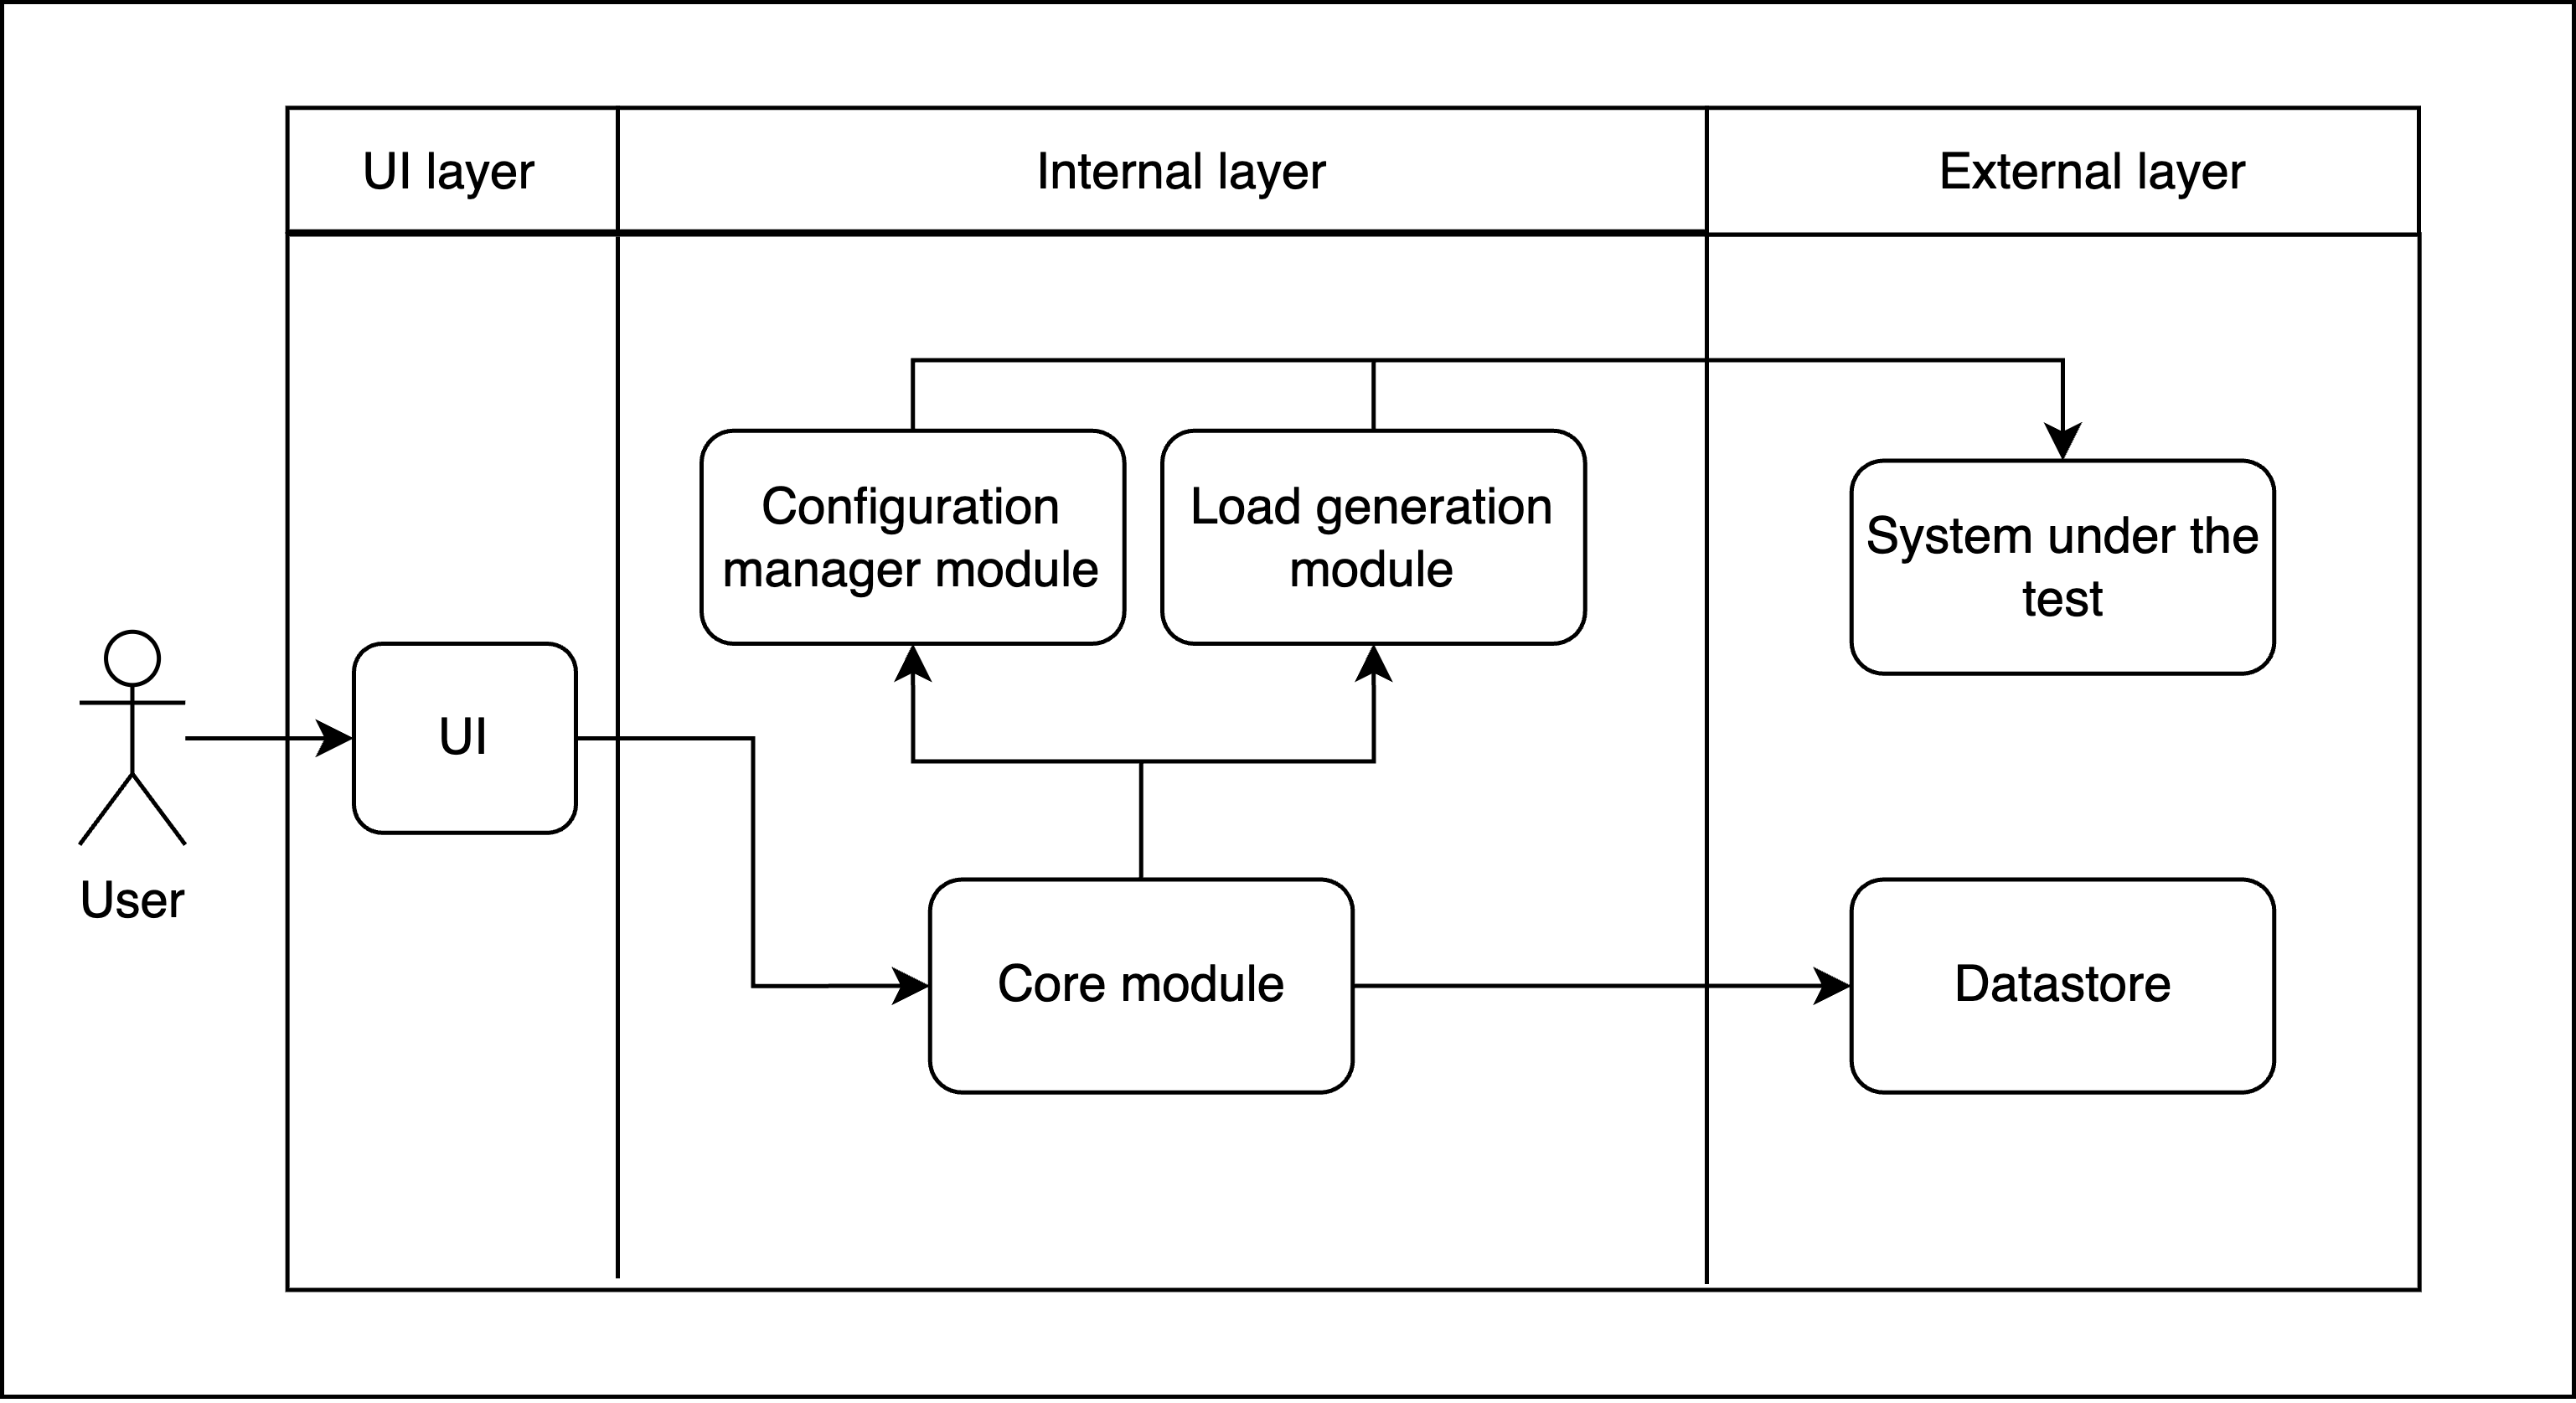
\includegraphics[height=\textheight,width=\textwidth,keepaspectratio]{design.png}
    \caption{System design}
    \label{fig:design}
\end{figure}

\subsection{UI layer}\label{subsec:ui_layer}
Needs to meet the functional requirement~\ref{subsec:fr:store_results}.
It should be able to visualize:
\begin{enumerate}
    \item List of scenarios. It should be provided in the form of a table, with the ability to sort the data by any column.
    \item Results of the executions. It should be presented in the form of charts, with the ability to add new charts or modify existing ones.
\end{enumerate}

\subsection{Internal layer}\label{subsec:internal_layer}
It should contain the main logic of the system for managing scenarios of testing. It is divided into:
\begin{enumerate}
    \item Orchestrator module. Needs to meet the functional requirement~\ref{subsec:fr:reproduce}. It should communicate with other modules and datastore to properly store and reproduce scenarios.
    \item Load generation module. Needs to meet the functional requirement~\ref{subsec:fr:execute_load_test}. It should provide an API for executing load tests and generating results in time series format.
    \item Configuration manager module. Needs to meet the functional requirement~\ref{subsec:fr:integrate}. It should be able to provide an API for reading and updating the configuration of the tested system.
\end{enumerate}

\subsection{External layer}\label{subsec:external_layer}
It should contain external services for the system. This layer is referred to as external because any component within it can be easily replaced. It is divided into:
\begin{enumerate}
    \item \textbf{Datastore}. Needs to meet the functional requirement~\ref{subsec:fr:store_scenarios}. It should provide an API for storing the scenarios and the results of their executions.
    \item \textbf{System under the test}. Any system that we want to test in different states of configuration.
\end{enumerate}